\documentclass[solution,addpoints,12pt]{exam}
\printanswers
\usepackage{amsmath,amssymb}

\newcommand{\RP}{\ensuremath{\mathsf{RP}}}
\newcommand{\expect}[1]{\ensuremath{\mathbb{E}[#1]}}
\newcommand{\dx}{\mathrm{d}x}
\usepackage{lmodern}
\usepackage{hyperref}
\hypersetup{
    colorlinks=true,
    linkcolor=blue,
    filecolor=magenta,      
    urlcolor=cyan,
}

\usepackage{graphicx}
\graphicspath{ {./images/} }


\begin{document}

\hrule
\vspace{3mm}
\noindent 
{\sf IITM-CS6024 : Algorithmic Approaches to Computational Biology  \hfill Date: Oct 4}
\vspace{3mm}\\
\noindent 
{\sf Assignment 4 \hfill Due Date : Oct 12, 23:55 }
%{\sf ~\hfill }
\vspace{3mm}
\hrule
\vspace{3mm}
\noindent{{\sf Roll No}: BE16B002 \hfill  {\sf Name}: Anoubhav Agarwaal }\\% ROLL NO AND DATE HERE
{{\sf Collaborators : Rahul Nikam}} %Names of the collaborators (if any).

%{{\sf References:}} %Reference materials, if any.
\vspace{3mm}
\hrule

\begin{questions}


\question[5] {[BWT]}: Let BWT and BWM refer to the Burrows-Wheeler Transform and Matrix respectively. 
\begin{parts}
\part[1] Reconstruct the string $S$ whose BWT($S$)~=~$nco\$toovican$ . 
\begin{solution}
The string is convocation\$. The lexicographically sorted BWM(S) is given by:
\begin{eqnarray*}
\begin{aligned}
\$convocatio\textbf{n}\\
ation\$convo\textbf{c}\\
cation\$conv\textbf{o}\\
convocation\textbf{\$}\\
ion\$convoca\textbf{t}\\
n\$convocati\textbf{o}\\
nvocation\$c\textbf{o}\\
ocation\$con\textbf{v}\\
on\$convocat\textbf{i}\\
onvocation\$\textbf{c}\\
tion\$convoc\textbf{a}\\
vocation\$co\textbf{n}\\
\end{aligned}
\end{eqnarray*}
The bold letters represent the BWT(S).
\end{solution}

\part[2] Find a string $T$ distinct from the above string $S$ such that BWM($T$) agrees with BWM($S$) on its $2^{nd}$ column (and possibly other columns).
\begin{solution}
For the BWM(T) to agree with the BWM(S) on its $2^{nd}$ column, the set of 2-mers of the strings S and T must be the same. For it to agree on the first k-columns, the k-mers of both the strings must be the same. 

The string T which has the same 2-mers as S can be obtained by finding the eulerian path in the De Bruijn graph constructed using the 2-mers of convocation\$, i.e., S. The De Bruijn graph (in the form of an adjacency list) is given by:
\begin{eqnarray*}
\begin{aligned}
a &-> t\\
c &-> a,o\\
i &-> o\\
n &-> \$,v\\
o &-> c,n,n\\
t &-> i\\
v &-> o\\
\end{aligned}
\end{eqnarray*}
The only other possible eulerian path (It must start and end with nodes of odd degree) in the graph is catioconvon\$.
The lexicographically sorted BWM(T = catioconvon\$) is given by:
\begin{eqnarray*}
\begin{aligned}
\textbf{\$c}atioconvon\\
\textbf{at}ioconvon\$c\\
\textbf{ca}tioconvon\$\\
\textbf{co}nvon\$catio\\
\textbf{io}convon\$cat\\
\textbf{n\$}catioconvo\\
\textbf{nv}on\$catioco\\
\textbf{oc}onvon\$cati\\
\textbf{on}\$catioconv\\
\textbf{on}von\$catioc\\
\textbf{tio}convon\$ca\\
\textbf{vo}n\$catiocon\\
\end{aligned}
\end{eqnarray*}
We observe that the BWM(S) and BWM(T) agree on the first two columns (compare with (a)).
\end{solution}

\part[2] Find a string $T'$ distinct from the above string $S$ such that BWM($T'$) agrees with BWM($S$) on its $2^{nd}$ and $3^{rd}$ columns (and possibly other columns). 
\begin{solution}
The 3-mer composition of the strings $T'$ and $S$ need to be the same. Such a string can be obtained by finding the eulerian path in the De Bruijn graph constructed using the 3-mers of convocation\$, i.e., string $S$. \\The De Bruijn graph (in the form of an adjacency list) is given by:
\begin{eqnarray*}
\begin{aligned}
at &-> ti\\
ca &-> at\\
co &-> on\\
io &-> on\\
nv &-> vo\\
oc &-> ca\\
on &-> n\$,nv\\
ti &-> io\\
vo &-> oc\\
\end{aligned}
\end{eqnarray*}
We observe that only one Eulerian path is possible in this graph, which corresponds to string $S$. Thus, no distinct string $T'$ exists such that BWM($T'$) agrees with BWM($S$) on its $2^{nd}$ and $3^{rd}$ columns 
\end{solution}
\end{parts}

\question[5] {[ST, SA and Substrings]}: Let SA and ST refer to suffix array and suffix tree respectively. 
\begin{parts}
\part[1] Briefly describe an algorithm that uses ST to find the longest substring shared by two strings.\\
(Bonus: How about a ST-based algorithm for finding the shortest substring of one string that does not appear in another string?)  
\begin{solution}
Let M and N be the two given strings of length m and n respectively. Brief Algorithm:
\begin{enumerate}
\item Build a suffix tree of a new combined string $M\#N\$$. Here, $\#$ and $\$$ are unique terminal symbols. This takes $O(m+n)$ time.
\item Annotate each internal node in the tree with either M, N, or MN. The internal node is annotated as M if it only consists of leaf nodes from string M. Similarly for N. The internal node is annotated MN if it has leaves from both the strings. This takes $O(m+n)$ time using DFS.
\item Run a DFS over the tree to find the deepest internal node labeled as MN. This is also in linear time.
\end{enumerate}
\end{solution}

\part[2] A linear-time algorithm to transform the   SA of a $n$-length string to its ST is possible with an auxiliary LCP array, which stores the length of the longest common prefix (lcp) of all pairs of consecutive suffixes in a sorted suffix array. That is, for $i=1\ldots n$, LCP[i] = length(lcp(suffix starting at position SA[i-1] in string, suffix starting at position SA[i] in string)). Can you design an $\mathcal{O}(n)$ algorithm to construct the LCP array of a string from its SA?
\begin{solution}
Let $SA$ be the suffix array of text $T$. Let's define the inverse suffix array $SA^{-1}$ which is the lexicographic rank of the suffix $T_j$, i.e., $SA^{-1}[SA[i]] = i$ for all $i \in [0..n].$\\
For LCP construction in linear time, we use the following \textbf{Lemma}: \\For any  $i \in [0..n)$, $LCP[SA^-1[i]]\ge LCP[SA^-1[i-1]] - 1$\\

\textbf{Problem}: LCP array construction\\
\textbf{Input}: text $T[0..n]$, suffix array $SA[0..n]$, inverse suffix array $SA^-1[0..n]$\\
\textbf{Output}: LCP array $LCP[1..n]$
\begin{enumerate}
\itemsep0em 
\item $l \leftarrow 0$
\item for $i \leftarrow 0$ to $n-1$ do
\item 	\quad $k \leftarrow SA^-1[i]$
\item 	\quad $j \leftarrow SA[k - 1]$
\item 	\quad while $T[i + l] = T[j + l]$ do $l \leftarrow l + 1$
\item 	\quad $LCP[k] \leftarrow l$
\item 	\quad if $l > 0$ then $l \leftarrow l - 1$
\item return $LCP$
\end{enumerate}
Proof that run-time is $O(n)$:\\(1) All steps other than 5 clearly take either constant or linear time.\\(2) Each round in the loop increments $l$.  Since $l$ is  decremented at most  $n$ times on line 7 and cannot  grow  larger than n,  the loop  is executed $O(n)$ times in total.\textsuperscript{\cite{q4c}}
\end{solution}

\part[2] The DC3 algorithm for SA construction (recursively) sorts suffixes starting at positions that are {\bf not} multiples of $3$ in the first step, and uses it to sort/merge suffixes that are at multiples of $3$ in later steps. What will happen if you extend this idea to get a DC2 algorithm (which sorts odd-position suffixes in the first step, and  uses it to sort/merge even-position suffixes in the next steps)? That is, will the DC2 algorithm steps be ``easier or trickier'' to implement than the DC3 algorithm steps? Justify briefly.\\
(Bonus: What subset of suffixes will you sort in the first step of a DC7 algorithm to get an algorithm similar to the DC3 algorithm?)
\begin{solution}
The DC2 algorithm will be trickier to implement compared to the DC3 algorithm in the later steps.
\end{solution}
\end{parts}


\question[10]{[Coding Time]}: Neighbor-Joining (NJ) is a quite popular bioinformatics algorithm with 30,000+ citations making it one of the top 20 most cited papers in all fields of science! 

\begin{parts}
\part[8] Solve the contest at \url{https://www.hackerrank.com/cs6024assignment-4} by implementing NJ to reconstruct a phylogenetic tree from a distance matrix. Please follow the instructions given carefully to produce the exact same output as the test cases.
%\begin{solution}
%In HackerRank.
%\end{solution}

\part[2] In your algorithm, you could've used n=3 instead of n=2 leaves as base case in recursion.  Related to this, prove that every $3 \times 3$ distance matrix is additive.
\begin{solution}
Let $d_{ij}(T)$ represent the distance between $i$ and $j$ in the tree T. Let D be a $3 \times 3$ distance matrix for 3 species $i, j,$ and $k$ such that $D_{ij} = x$, $D_{jk} = y$, $D_{ki} = z$. Here, $D_{ij}$ represent entries in the distance matrix.\vspace{1mm}\\
To Prove: Every 3x3 matrix is additive, i.e., there exists a tree T with\\ $d_{xy}(T) = D_{xy} \forall$ $ x, y$ \hspace{10mm}                (1)\vspace{1mm}\\
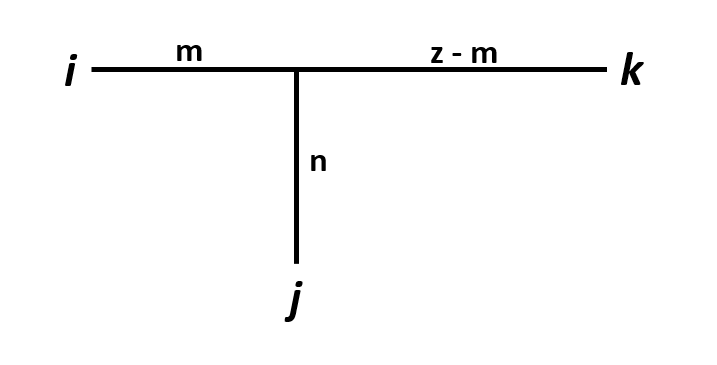
\includegraphics[scale = 0.7]{pic}\\
(Refer to figure) WLOG, Connect the nodes of the tree $i$ and $k$ with an edge of length $D_{ik}$, i.e., $d_{ik} = D_{ik} = z$. Take any point at a distance of $m$ from $i$ on this edge. From this point let species $j$ be at a distance of $n$. \vspace{1mm}\\
For condition (1) to hold and thus the a general $3 \times 3$ matrix to be additive, the following equations need to be satisfied:
\begin{eqnarray*}
\begin{aligned}
d_{ij} &= D_{ij} = x\\
d_{ij} &= m + n = x \hspace{30mm} (i)\\
d_{jk} &= D_{jk} = y\\
d_{jk} &= z - m + n = y \hspace{25mm} (ii)\\
\end{aligned}
\end{eqnarray*}
Equations (i) and (ii) are a system of two linear equations with two unknowns $m$ and $n$. The equations are always solvable. The solution is give by: 
\begin{eqnarray*}
\begin{aligned}
m &= (x + z - y)/2\\
n &= (x - z + y)/2\\
\end{aligned}
\end{eqnarray*}
Hence, for any $3 \times 3$ distance matrix, we can obtain its corresponding tree.
\end{solution}
\end{parts}

\question[10] {[Research critique]}:
Please provide critique on the research paper assigned to you (students are randomly assigned another team's paper to critique; please find your paper from the 
\href{https://docs.google.com/spreadsheets/d/1FOjMSlAX676ZlyV_A2tndzjcGv6TIvVn9NMnLgh-dJw/edit?usp=sharing}{allotment file here}).

\begin{parts}
\part[3] Please provide a brief overview of the paper in the format described.
(Format: Mention the (i) biological question addressed in the paper, (ii) computational problem (in the same format as in the textbook/lecture-slides) studied in the paper, and (iii) computational methods/approach taken to solve the problem.)
\begin{solution}Paper Title: Novel risk genes for systemic lupus erythematosus predicted by random forest classification.\\
(i) \textbf{Biological question}\\
Systemic lupus erythematosus is an autoimmune disease whereby the immune system of the body attacks its healthy cells. The disease is characterized by inflammation of organs. There is no cure available to treat SLE completely. Treatment options involve bettering quality of life and alleviating symptoms.
As SLE is a genetic disease, people can be at a predetermined risk of getting the disease. To identify the genetic components that play a part in the disease and to identify novel genes that are implicated in SLE, the study uses machine learning algorithms for better prediction. To further validate the data, the expression patterns of B-cells and T-cells are studied for the identified genes, and their regulatory mechanisms are investigated to study cell-dependent genetic contributions. 
\vspace{3mm}\\
(ii) \textbf{Computational problem}
\begin{enumerate}
\itemsep0em 
\item Random Forest Classifier
\item Logistic Regression
\end{enumerate}
The paper investigates the difference in prediction accuracy in the above-mentioned models for the same datasets. These two models are also used to predict the risk for Lupus Nephritis, a severe manifestation of SLE. 
\vspace{1mm}\\
Input: SNP genotype data\\
Output: Gini importance score and Probability value
\vspace{3mm}\\
(iii) \textbf{Computational method}\\
The paper implements a Random Forest classifier to predict SLE risk and identify genes that might be involved in conferring SLE risk in individuals.\\
R package used: EMIL (Evaluation of Modeling without Information Leakage)\\
The status prediction was performed with 15 fold cross-validation runs involving 3000 SNPs per classification fold.
\end{solution}

\part[3] Mention three strengths or key contributions of the paper in your own words (not copied as is from paper). 
\begin{solution}
The key contributions of the paper are:
\begin{enumerate}
\item The paper designed a random forest classifier to predict whether a person is at risk of SLE. Random forest was able to give a better prediction accuracy, with an AUC score of 0.78. Furthermore, they were able to give better prediction accuracy when a severe form of SLE, lupus nephritis, was used as a test case. 
\item The investigating team genotyped many individuals from Sweden and collected their SNP information. This genotyped data was comparable with the GWAS catalog in terms of the predicted genes. 
\item The classifier was able to identify 3 novel genes to be implicated in SLE. These 3 genes haven’t been previously indicated in SLE. The genes have a high gene importance score denoted by RF classifier. Moreover, these genes rank alongside 37 other genes, some of which have been implicated in SLE by GWAS studies. Similarly, they were able to identify 6 novel genes implicated only in Lupus Nephritis.
\item After identifying genes that may play a role in SLE, they studied the expression patterns of the genes. This study further helps validate the functional roles of the novel genes. They furthermore studied whether B-cells or T-cells contain the overexpressed genes and studied the gene expression preference between the two. This analysis not only helps understand the expression of genes but also highlights the importance of cell-specific expression analysis to understand the disease better. Furthermore, the paper also investigates the transcriptional regulation mechanism of the top 40 genes. Hence the paper has firmly established their findings with genetic and gene expression findings along with information about the cis-regulatory elements. 
\end{enumerate}
\end{solution}

\part[3] Mention three areas of further improvement of the paper.\\
(Note: If it is a theoretical paper, state whether the proofs were easy to read, if there was clarity in the presentation, etc. It there is empirical investigation, you can comment about the results obtained, if those results mentioned can be replicated or improved using some other idea you have. You can also write about the gaps in the paper, and ideas you may've about filling those gaps.)
\begin{solution} Areas for further improvement of the paper:
\begin{enumerate}
\item While random forest for SLE gives a prediction accuracy of 0.78, which is an improvement over logistic regression, it hasn’t been mentioned why this difference exists. Moreover, SLE lupus nephritis gives an AUC score of 0.91, which is the highest score obtained. No explanation as to why this result gives a better prediction accuracy only for the RF classifier has been given. Further enhancements to improve the SLE prediction accuracy have not been explored. 
\item Comparisons with more models like Bayes classifier will help understand why/why not RF classifier works best. No previous work has been cited for the same. 
\item The study investigates the cell-specific regulation and preferences of gene expression. In the study, the top 40 genes show a significant over-expression in T-cells compared to B-cells. Moreover, there are more B-cell specific genes than T-cell specific genes in the top 40 identified genes. The reason for this hasn’t been explored. In an autoimmune disease, there are more immune cells that play an essential part in carrying out an immune attack. Why these specific identified genes show enriched B-cell expression and not T cell needs to be further explored. Along with this, the genes expressed in T-cell and associated with SLE need to be identified. Similar studies should be extended to Lupus Nephritis for functional validation.
\end{enumerate}
\end{solution}

\part[1] Considering both above, please mention whether the work is a significant contribution to this field.
\begin{solution}
The work conducted is significant as it lays the groundwork for the use of machine learning techniques for a complex disease like SLE. It also investigates cell-specific gene expression as well as the genetic factors of the disease. However, more work is required to identify more genes and improve the prediction of risk status for other demographics, with the use of other genotyping and machine learning tools.
\end{solution}
\end{parts}


\bibliographystyle{ieeetr}
\bibliography{References}

\end{questions}
\end{document}
